% Framework architecture. Compile on its own: pdflatex architecture.tex
\documentclass[tikz,border=2pt]{standalone}
\usepackage[T1]{fontenc}
\usetikzlibrary{positioning,arrows.meta,fit}
\begin{document}
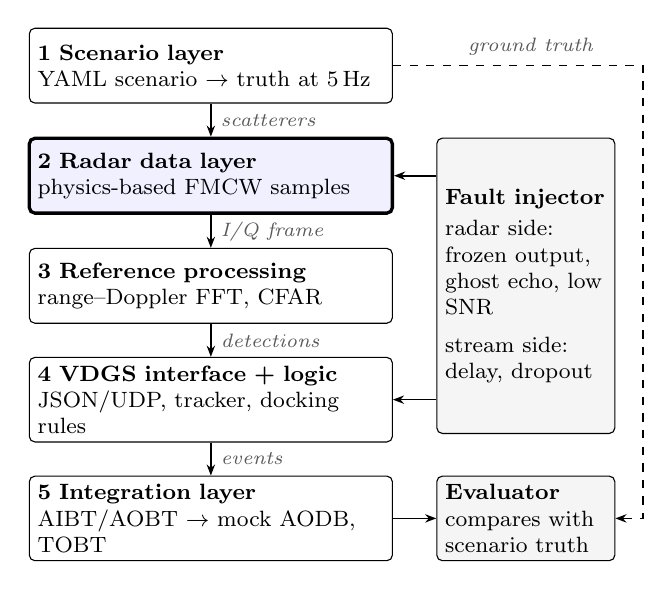
\begin{tikzpicture}[
  font=\footnotesize,
  layer/.style={draw, rounded corners=2pt, minimum width=4.6cm, minimum height=0.95cm,
                align=left, text width=4.4cm, inner sep=3pt},
  core/.style={layer, very thick, fill=blue!6},
  side/.style={draw, rounded corners=2pt, align=left, text width=2.05cm, inner sep=3pt, fill=black!4},
  arr/.style={-{Stealth[length=4pt]}, semithick},
  lbl/.style={font=\scriptsize\itshape, text=black!65}
]
\node[layer] (s) {\textbf{1 Scenario layer}\\ YAML scenario $\rightarrow$ truth at 5\,Hz};
\node[core, below=0.42cm of s] (r) {\textbf{2 Radar data layer}\\ physics-based FMCW samples};
\node[layer, below=0.42cm of r] (p) {\textbf{3 Reference processing}\\ range--Doppler FFT, CFAR};
\node[layer, below=0.42cm of p] (i) {\textbf{4 VDGS interface + logic}\\ JSON/UDP, tracker, docking rules};
\node[layer, below=0.42cm of i] (a) {\textbf{5 Integration layer}\\ AIBT/AOBT $\rightarrow$ mock AODB, TOBT};

\draw[arr] (s) -- node[right, lbl] {scatterers} (r);
\draw[arr] (r) -- node[right, lbl] {I/Q frame} (p);
\draw[arr] (p) -- node[right, lbl] {detections} (i);
\draw[arr] (i) -- node[right, lbl] {events} (a);

\node[side, right=0.55cm of p, minimum height=3.75cm] (f) {\textbf{Fault injector}\\[2pt] radar side: frozen output, ghost echo, low SNR\\[4pt] stream side: delay, dropout};
\draw[arr] (f.west |- r.east) -- (r.east);
\draw[arr] (f.west |- i.east) -- (i.east);

\node[side, right=0.55cm of a] (e) {\textbf{Evaluator}\\ compares with scenario truth};
\draw[arr] (a) -- (e);
\coordinate (gx) at ([xshift=0.35cm]e.east);
\draw[arr, dashed] (s.east) -- node[above, lbl, pos=0.55] {ground truth} (s.east -| gx) -- (gx) -- (e.east);
\end{tikzpicture}
\end{document}
